%%%%%%%%%%%%%%%%%%%%%%%%%%%%%%%%%%%%%%%%%%%%%%%%%%%%%%%%%%%%%%%%%%%%%%%%%%%%%%%%
%2345678901234567890123456789012345678901234567890123456789012345678901234567890
%        1         2         3         4         5         6         7         8
% THESIS CHAPTER

\chapter{The algorithms}
\label{chap:algorithms}
\ifpdf
    \graphicspath{{Algorithms/Figures/PNG/}{EvaluationTask/Figures/PDF/}{Algorithms/Figures/}}
\else
    \graphicspath{{Algorithms/Figures/EPS/}{EvaluationTask/Figures/}}
\fi


% short summary of the chapter
The main algorithms analysed in the project are attempted to be as different as
possible from each other. This allows covering as many audio features and
similarity measuring techniques as possible. My motivations of the choice of
algorithms were influenced by the study on MIREX submissions, as well as the
overall scope of features they encompass. 

Julien Osmalsky coins the term \textit{rejector} to define a pairwise comparison
function that given two audio tracks it returns a score ranking of similarity
between both tracks \cite{osmalsky2015combining}. This term was adopted by the
project to refer to each of the algorithms examined. The relation between an
algorithm paper and its rejector term is outlined in section \ref{sec:algolist}.

The final selection includes 5 individual algorithms and an algorithm
aggregating results from 4 of them. Each of the algorithms is examined
individually, with the results from some of them combined through the rank
aggregation algorithm.


\section{Algorithms list}
\label{sec:algolist}
The analysis if performed on the following algorithm:
\begin{itemize}
    \item \textbf{Weak rejector} - Osmalskyj, Julien, Marc Van Droogenbroeck,
    and Jean-Jacques Embrechts. \textit{Enhancing cover song identification with
    hierarchical rank aggregation} \cite{osmalsky2016enhancing}
    \item \textbf{Cross-correlation rejector} - Ellis, Daniel PW, Courtenay V.
    Cotton, and Michael I. Mandel. \textit{Cross-correlation of beat-synchronous
    representations for music similarity} \cite{ellis2008cross}
    \item \textbf{Quantisation rejector} - Osmalskyj, Julien, et al.
    \textit{Combining features for cover song identification} \cite{osmalsky2015combining}
    \item \textbf{Timbre rejector} - Tralie, Christopher J., and Paul Bendich.
    \textit{Cover song identification with timbral shape sequences} \cite{tralie2015cover}
    \item \textbf{Aggregated rank rejector} - Osmalskyj, Julien, Marc Van
    Droogenbroeck, and Jean-Jacques Embrechts. \textit{Enhancing cover song
    identification with hierarchical rank aggregation}
    \cite{osmalsky2016enhancing} 
    \item \textbf{Fingerprint rejector} - Rafii, Zafar, Bob Coover, and Jinyu
    Han. \textit{An audio fingerprinting system for live version identification
    using image processing techniques} \cite{rafii2014audio}
\end{itemize}

\begin{figure}[H]
    \centering
    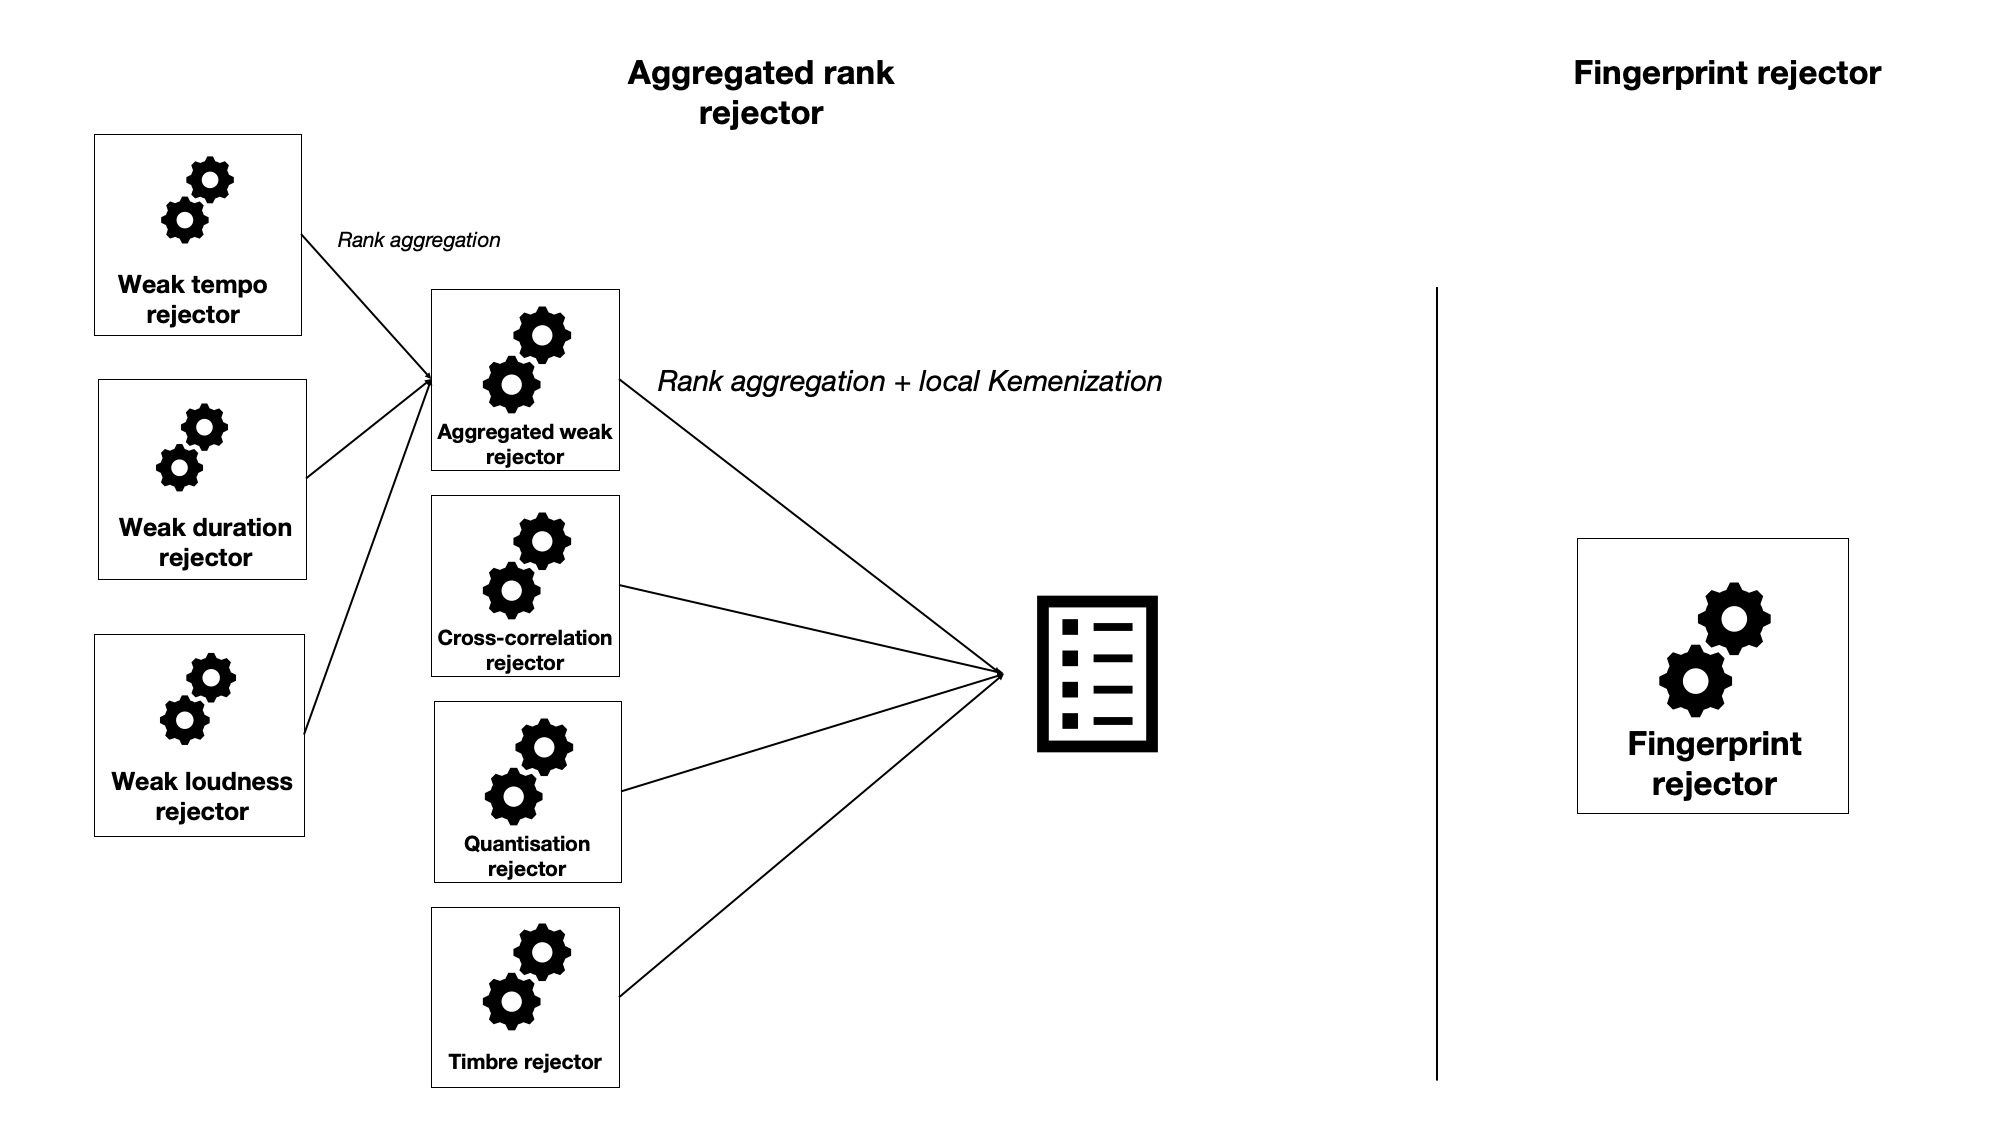
\includegraphics[width=\textwidth]{Algorithms/algorithm_diagram_3.jpg}
    \captionof{figure}[Algorithms diagram]{Diagram of chosen algorithms and the relationships between them. The aggregated rank rejector combines the results of 3 types of weak rejectors, as well as the quantisation, cross-correlation and timbre rejectors}
    \label{fig:algorithms}
\end{figure}

\section{Weak rejector} 
\label{sec:osmalskyj}

The weak rejector takes its name from the fact that it uses global single-valued
features of sound to calculate a similarity score. Weak features include tempo,
duration, loudness, average number of beats, etc. Those audio properties are
considered 'weak' since by themselves they cannot uniquely describe a song - the
majority of pop tracks from a certain era are composed with the same tempo, for
example \cite{slowpop}. As a consequence the results from weak rejectors are
inherently insignificant are usually not considered individually, but as
part of an aggregation with other results.

Each weak rejector takes a single audio feature as song representation. The
algorithm extracts the feature from each song in a dataset and from them it
creates a training set by combining each pair of songs in different ways. For
songs $A$ and $B$ with weak feature values of $f1$ and $f2$ respectively the
minimum ($min(f1, f2)$), maximum ($max(f1, f2)$), sum ($f1 + f2$), quotient
($\frac{f1}{f2}$) and absolute value of quotient of the difference divided by
the sum ($abs(\frac{f1 - f2}{f1 + f2})$) are taken. The generated data is used
as attributes to train an ExtraTrees classifier model. Extra randomised trees or
ExtraTrees classification is a form of random forest classification. In
contrast to the regular random forest implementation, ExtraTrees uses the whole
training data for each decision tree. Rather than calculating an optimal
cut-point, it also uses a random one. The direct benefits of using this
variation of random trees are higher computational efficiency while achieving
similar perfomance on average, in addition to better results on some specific
problems \cite{geurts2006extremely}.

The evaluation datasets used in this project are too small to generate an
ExtraTrees model which performs even adequate classification of songs. To gather
sufficient training data the weak features of 12,104 songs are extracted from
the music streaming service Spotify \cite{spotify}. The tracks are chosen based
on clique groupings from the SecondHandSongs (SHS) \cite{shs} dataset - the
largest dataset of covers songs aimed at academic research. While the full
dataset is difficult to obtain, information about the cliques structure within
it is easy to find. The extracted data is then combined into pairs using the
procedure outlined in the previous paragraph. A binary class is then assigned to
each pair entry depending on whether the pair of songs are covers or not.
Afterwards the training data is further split into a training set of 3773
cliques (8653 songs) and validation set containing 1573 cliques (3451 songs).
The metric used to validate the model performance is the area under the receiver
operating characteristic (ROC) curve - a curve resulting from the plot of the
true positive against the false positive rate of the validation results. ROC
analysis of such form is suitable as a validation metric for the selection of an
optimal model because it is independent of any potential cost function or cost
distribution \cite{wiki:roc}. Because we are solely working with weak feature
information the we can only validate based on correct and incorrect produced results.

After the training phase is complete each of the evaluation datasets is
converted into the training set format and passed to the model for class
prediction. The output result is a probability of every pair of songs being
covers. Grouping the results per song produces a database ordering that is
required by the evaluation task.

\section{Cross-correlation rejector} 
\label{sec:weakfeatures}
The cross-correlation rejector uses chroma features as the main audio feature
describing each song. Chroma is another name for pitch class profiles, i.e. a
12-dimensional representation of the intensity distribution in each of the
twelve pitch classes part of the chromatic scale \cite{fujishima1999real}. Any
feature that at its core uses chroma to represent a song is a chroma feature.
That is why the terms harmonic pitch class profiles (HPCP) and chroma features
have a very similar definition, in fact HPCP is a type of chroma feature. The
main difference between chroma features is their method of extraction. Using
chroma features produces a chromagram - a pitch class versus time plot showing
the intensity of each pitch class at any time point (Figure
\ref{fig:chromagram}).

\begin{figure}[H]
    \centering
    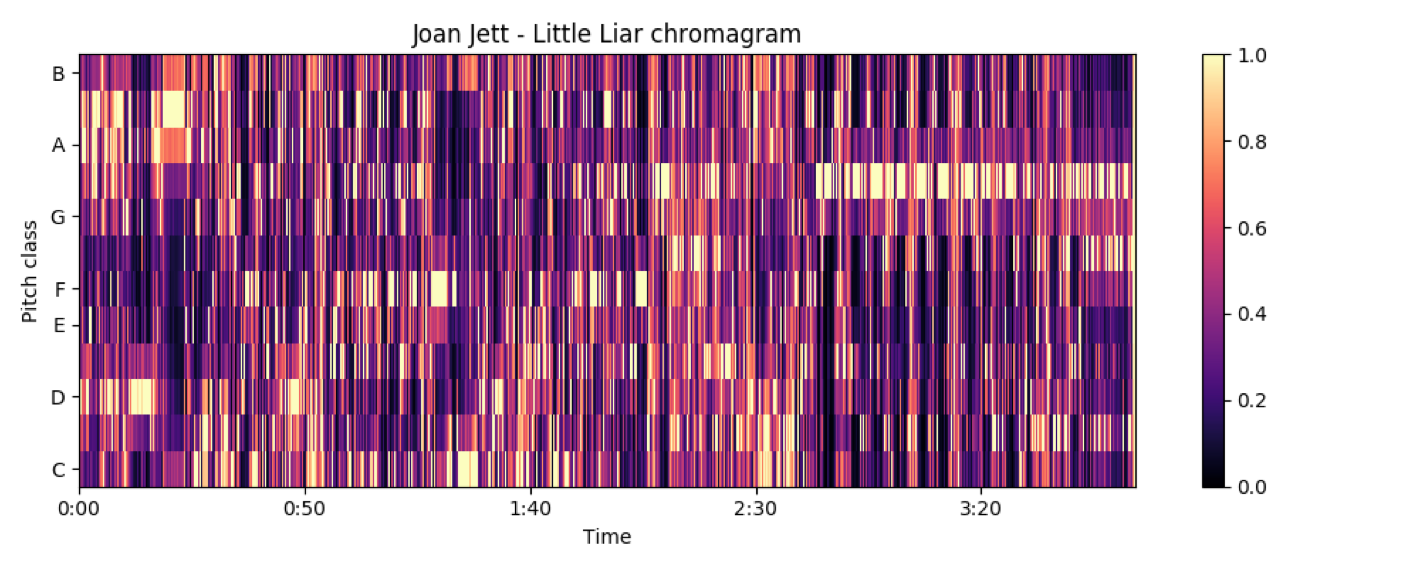
\includegraphics[width=\textwidth]{Algorithms/chromagram_picture.png}
    \captionof{figure}[Chromagram]{Chromagram of the song \textit{Little Liar} by Joan Jett}
    \label{fig:chromagram}
\end{figure}

The chroma features in the cross-correlation rejector are extracted by
performing short-time Fourier transform (STFT) analysis. It consists of running
Fourier transform on short segments of a signal to determine how the frequency
content changes over time \cite{gao2006non}. STFT improves upon the concepts of
regular Fourier transform by not only telling us what frequencies are contained
within the audio stream, but also at what time intervals does each frequency
appear.

The transformations are applied using the fast Fourier transform (FFT)
algorithm. The short segments are calculated over sliding overlapping windows as
illustrated on figure \ref{fig:stft}. The size of the sliding window is
determined by \textit{FFT window size} and the overlap between each window
depends on a parameter called \textit{hop length}. The actual window overlap is
calculated as the difference between the window size and the hop length.

\begin{figure}[H]
   \centering 
   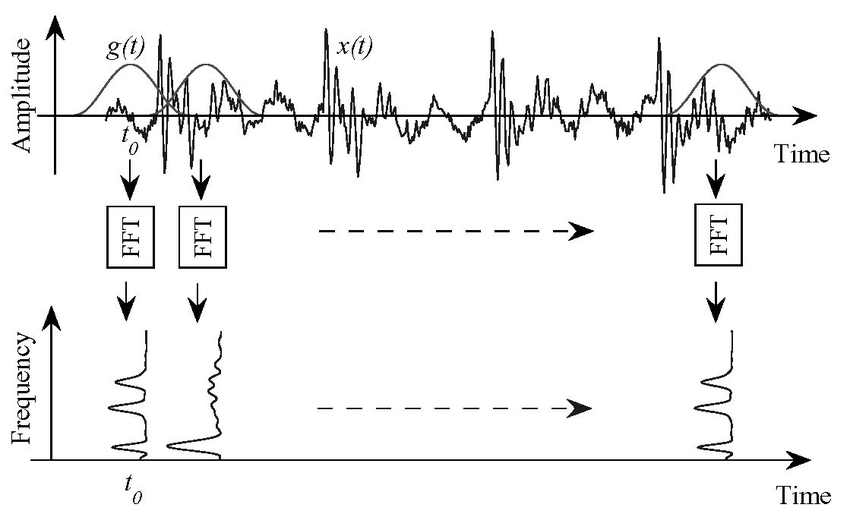
\includegraphics[width=\textwidth]{Algorithms/stft.png}
   \captionof{figure}[Short-time Fourier transform]{Workings of STFT on an audio signal $x(t)$. $g(t)$ is a function defined using the FFT window size and the hop length. The result of each FFT transformation is the amplitude and phase of frequency over the time period. \cite{gao2006non}}
   \label{fig:stft}
\end{figure}

The next step into obtaining chroma features for the cross-correlation rejector
is converting the spectrogram resulting from the STFT into a chromagram. Using
the standard mapping of pitch $A4 = 440 Hz$ and knowing that pitches in music
lay on an equal-tempered scale we can calculate the remaining pitches (relative
to A4) from the frequency spectrum.  We then aggregate all pitches belonging to
the same pitch class and that gives us the chroma value of the chroma value
corresponding to the class.

The conversion from frequency to pitch is regulated using a specification
defining a function to be used when the pitches relative to $A4$ are calculated.
This standardisation is commonly referred to as \textit{tuning standard}. The
paper describing the cross-correlation rejector does not specify what tuning was
used to generate the chroma features, so a library implementation of chroma
feature extraction was used in the benchmark. To further explain the conversion
of frequency to chroma an example using the \textit{MIDI tuning standard} is
presented. Figure \ref{fig:spectrotochroma} follows each stage of the procedure.

The MIDI tuning covers a range of 128 frequencies enumerated from 0 to 127. A4
(which again corresponds to $440 Hz$) is assigned number 69 and all other
pitches are calculated using the equation:

\begin{figure}[H]
    \label{fig:midiequation}
    \begin{equation}
       d = 69 + 12 \log_{2}(\frac{f}{440 Hz})
    \end{equation} 
    \captionof{figure}[MIDI Tuning pitch calculation equation]{Calculating pitch from frequency $f$ based on MIDI tuning standard \cite{mts}.}
\end{figure} 

This gives us a song representation similar to the one from
\ref{fig:spectrotochroma} c). The final step is to sum all MIDI pitch
coefficients into their corresponding pitch classes and obtain the chromagram
from \ref{fig:spectrotochroma} d).

\begin{figure}[H]
    \centering
    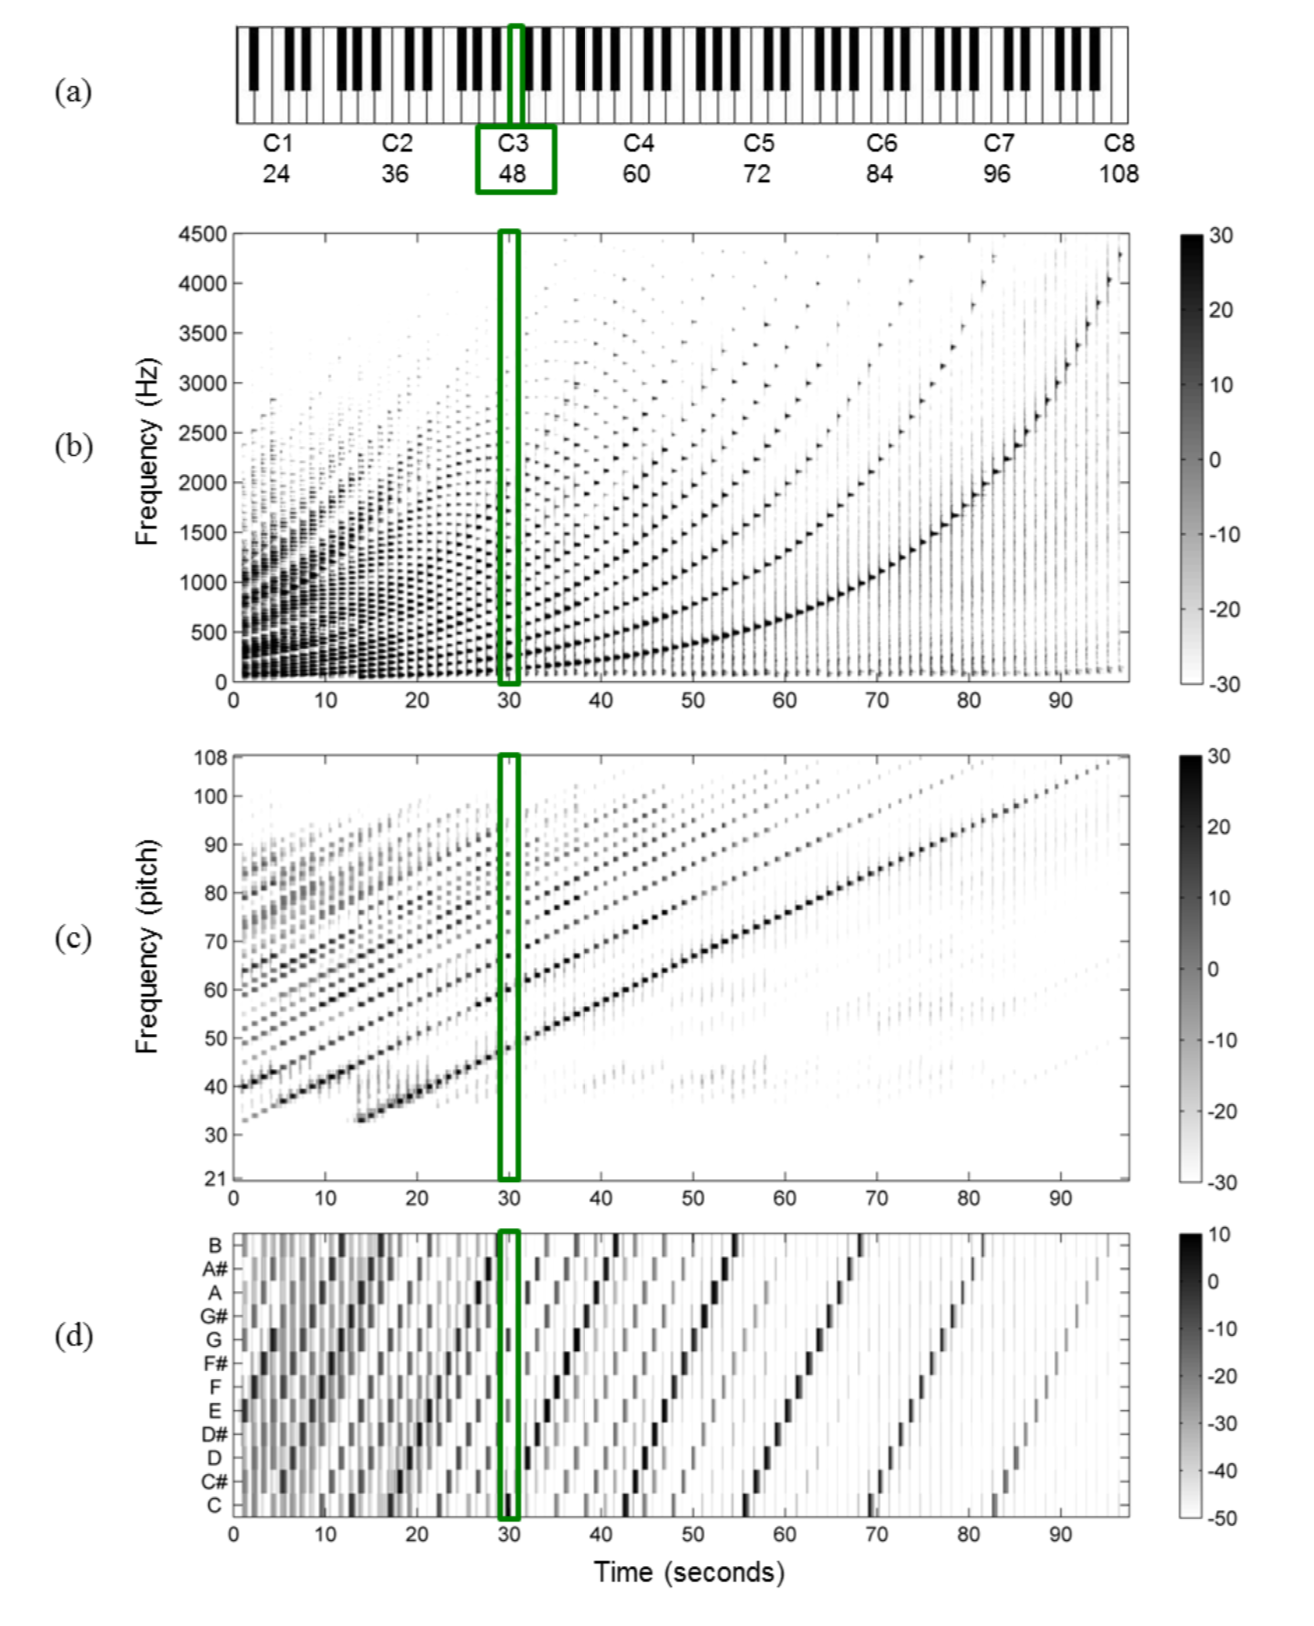
\includegraphics[width=0.69\textwidth]{Algorithms/spectrogram_to_chromagram.png}
    \captionof{figure}[Spectrogram to chromagram conversion]{The separate stages of a spectrogram to chromagram conversion of a piano recording of the chromatic scale from A0 to C8 using MIDI tuning. \cite{mullershort}. a) The equal-tempered scale represented by the keys of a piano, with the pitch C3 mapped to 48 according to MIDI Tuning b) A spectrogram of the song, with the time frame where C3 was played marked in red c) Pitch log-frequency representation of the spectrogram d) Resulting chromagram}
    \label{fig:spectrotochroma}
\end{figure}

\paragraph{}
The chroma features in the cross-correlation rejector are
\textit{beat-synchronous}. This means that the period over which a chroma
feature is obtained is every beat of the song, rather than a shorter time
segment. Understanding beat detection in detail was beyond my abilities and a
library implementation of a beat tracker created by the algorithm creators is
directly used to obtain a result \cite{librosa_beat}.

\paragraph{}
The resulting chromagrams for two songs are then scaled to unit length, so that
the sum of all dimensions of the chroma vector has a sum of 1. The
representation of the longer song is also shortened to be equal to the one of
the shorter song. The chromagram matrices are then cross-correlated. To account
for variations in the structure or pitch of the cover songs the shifts of the
chromagrams between -500\dots500 beats are considered. The resulting intervals
of peak values of peaks in the resulting cross-correlation matrix indicate a
strong match between both tracks. Figure \ref{fig:cross-correlation} shows the
correlation process of two chromagrams. The blue line in the cross-correlation
matrix indicates the strong similarity detected.

The similarity score that the rejector returns is the reciprocal value of the
highest peak value in the cross correlation matrix.

\begin{figure}
    \centering
    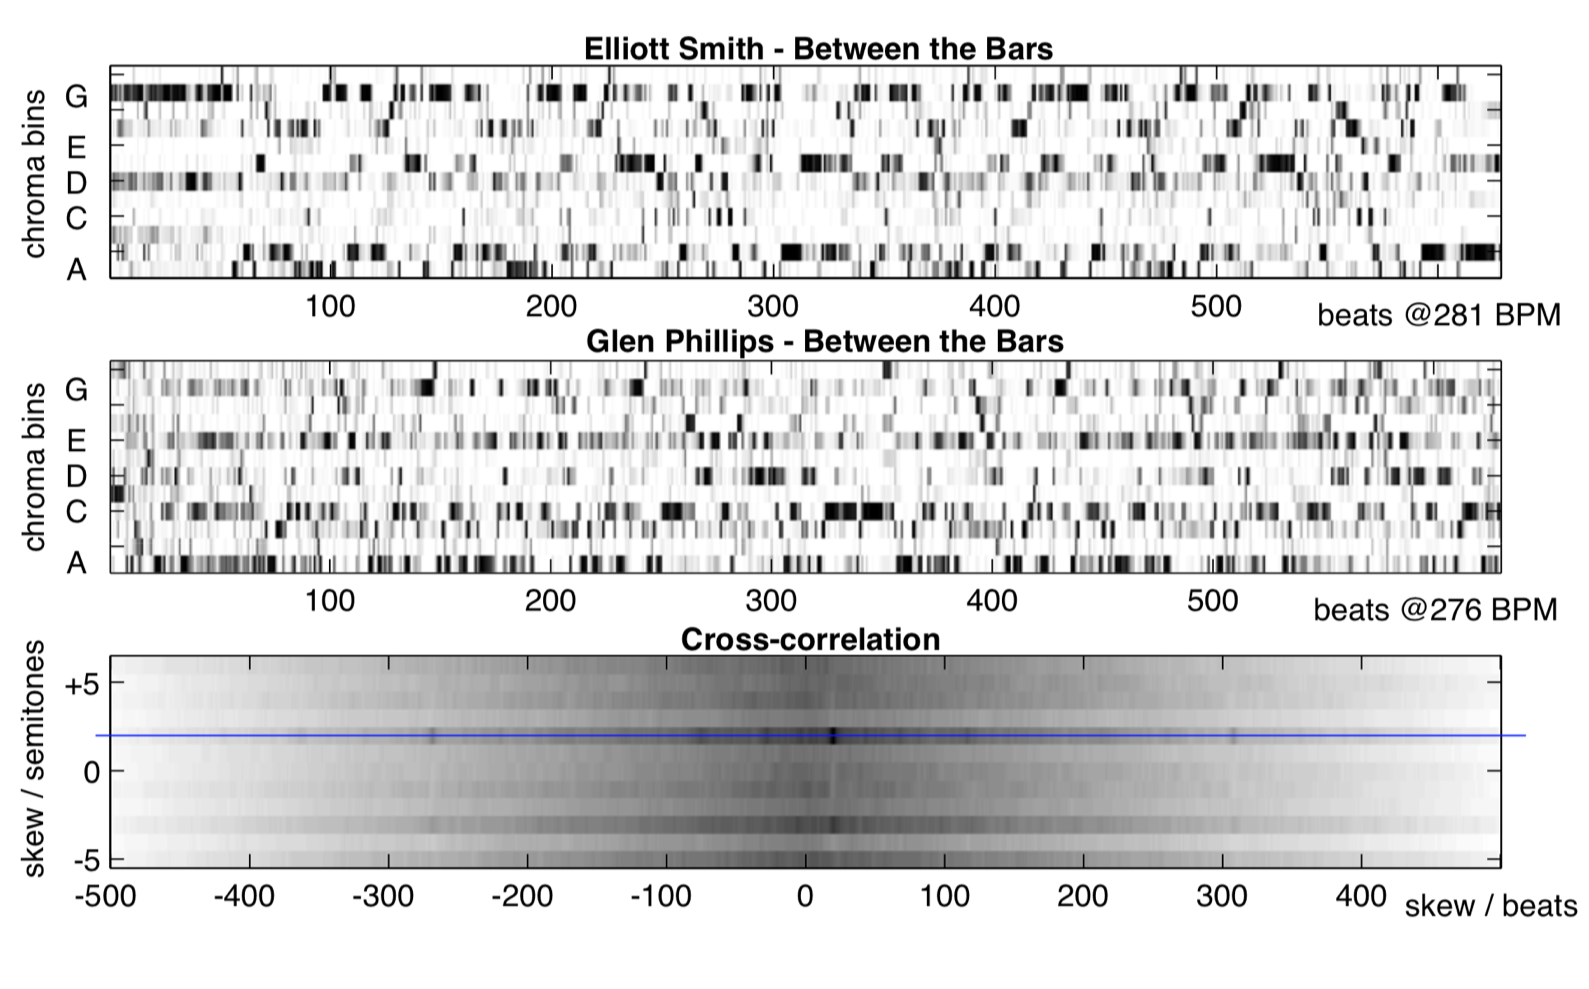
\includegraphics[width=\textwidth]{Algorithms/cross-correlation.png}
    \captionof{figure}[Cross-correlation of chromagrams]{Extracted chromagrams of two cover songs and the resulting cross-correlation \cite{ellis2007identifyingcover}}
    \label{fig:cross-correlation}
\end{figure}

\section{Quantisation rejector}
\label{sec:ccs}




\section{Timbre rejector} 
\label{sec:quantisation}
\section{Aggregated rank rejector} 
\label{sec:timbre}
\section{Fingerprint rejector} 
\label{sec:rankaggregation}

